\section{Arbres d'attaque et de défense}
	\label{sec:etat_art}

    \subsection{Méthodologie}
        Le concept des arbres d'attaque a été introduit en 1999 par Bruce Schneier, un expert américain en sécurité informatique qui est parti du constat que des systèmes réputés \og inviolables \fg se font briser en permanence \cite{doc_Schneier}. De plus, ces systèmes sont brisés par des méthodes d'accès qui n'avaient pas été imaginées par leurs concepteurs, car ils n'avaient pas les outils pour dresser une liste exhaustive des attaques possibles. Schneier a donc créé le concept des arbres d'attaque dans ce but : pouvoir réaliser un inventaire complet des méthodes d'attaque sur un système, quel qu'il soit, afin de pouvoir en concevoir la défense de la manière la plus adaptée. Schneier a lui-mêœme conçu son modèle d'arbre d'attaque à partir du principe des \og arbres de défaillances \fg, une méthodologie datant du début des années soixante dont le but est de pouvoir évaluer l'impact de la défaillance d'un composant sur son système \cite{defaillanceTree}.

        Lors de ses recherches, Schneier a retenu une représentation des menaces sous la forme d'arbres, expliquée par la Figure \ref{fig:arbre_exemple_1}. Ces arbres modélisent les pré-requis nécessaires à la réalisation de l'objectif principal (dans notre exemple, accéder au compte en banque d'une personne). Pour cela, on représente d'abord cet objectif à la racine de l'arbre, puis on le décompose en objectifs intermédiaires, appelés \og nœuds \fg. Ces derniers sont ensuite re-décomposés de la même façon en répétant l'opération autant de fois que nécessaire. Les nœuds de l'arbre d'attaque sont par convention représentés par des ovales reliés entre eux par des traits.

        \begin{figure}[h]
            \centering
            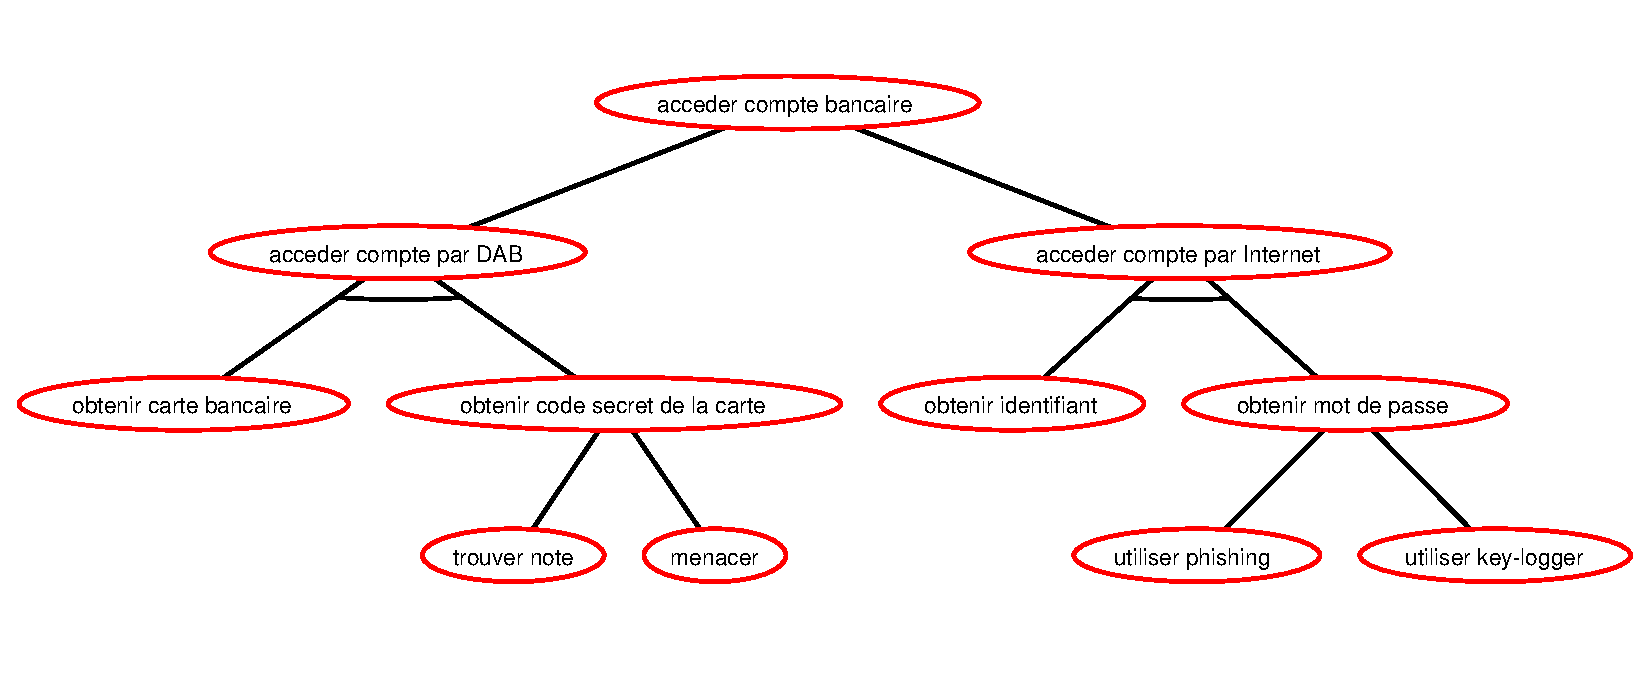
\includegraphics[width=1\textwidth]{figure/exemple1_rapport.pdf}
            \caption{Arbre d'attaque}
            \label{fig:arbre_exemple_1}
        \end{figure}

        La relation entre les fils d'un nœud peut prendre deux formes distinctes :
        \begin{itemize}

            \item la {\bf disjonction}, qui correspond au cas où la validation d'un seul nœud fils suffit à valider le nœud père. Cette relation équivaut à l'opération logique \og OU \fg{}. Dans notre exemple, accéder au compte en banque de quelqu'un peut se faire soit par un distributeur automatique de billets (DAB), soit par Internet.

            
            \item la {\bf conjonction}, qui correspond au cas où la validation de l'ensemble des nœuds fils est nécessaire pour valider le nœud père. Cette relation équivaut à l'opération logique \og ET \fg{}. On la représente par un arc de cercle reliant les relations père-fils. Par exemple, pour retirer de l'argent d'un compte bancaire depuis un DAB, il faut à la fois obtenir une carte bancaire et le code secret associé.
        \end{itemize} 
	

	\paragraph{}

        Enfin, le modèle des arbres d'attaque permet d'associer aux nœuds des paramètres représentant des informations quantitatives ou qualitatives sur l'action : coût, difficulté, probabilité, temps d'exécution, etc. Ces paramètres permettent de quantifier le poids du nœud dans l'arbre. Il est alors possible, en utilisant les fonctions appropriées, de propager ces paramètres au nœud père. Ceci permet à l'attaquant de choisir une stratégie d'attaque plutôt qu'une autre au vu de ses ressources. La Figure \ref{fig:arbre_exemple_2} illustre le coût monétaire minimum pour l'attaquant. On remarque dans ce cas précis que le coût d'un nœud disjonctif est le coût minimal de ses fils, tandis que le coût d'un nœud conjonctif en est la somme. Chaque quantification a un mode de calcul propre vis-à-vis du type de nœud (disjonctif ou conjonctif). Il est également possible de combiner plusieurs paramètres pour en produire de nouveaux. Par exemple, on peut obtenir le paramètre \og risque \fg{}  en multipliant la \og probabilité de succès\fg{} de l'attaque par son \og impact\fg{}.

        \begin{figure}[h]
	        \centering
	        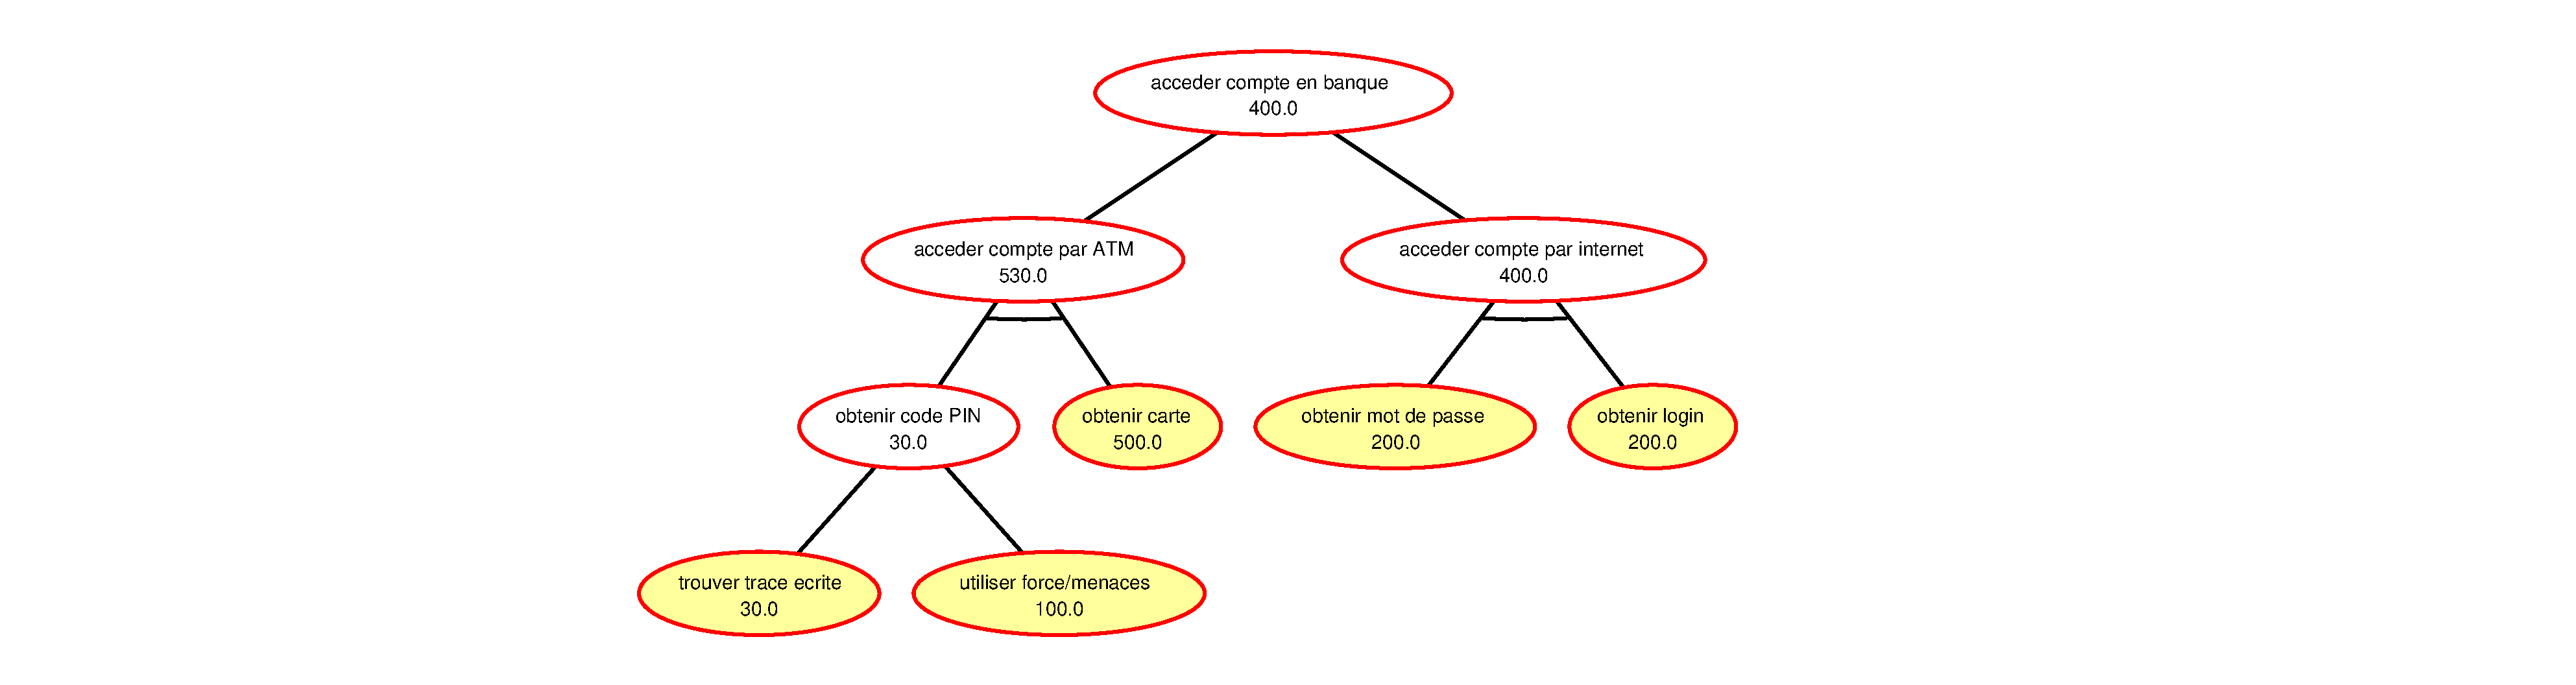
\includegraphics[width=1\textwidth]{figure/quantification.pdf}
	        \caption{Quantification du coût de l'attaque}
	        \label{fig:arbre_exemple_2}
        \end{figure}

		Le concept des arbres d'attaque a évolué grâce à la contribution de personnes ayant amélioré le modèle de Schneier \cite{ADTreeKordy}. En particulier, le concept d'arbre d'attaque a été étendu à celui d’arbre d’attaque et de défense (\og attack–defense tree \fg{} en anglais, ou \og ADTree \fg{}). Les ADTrees représentent non seulement les (sous-)objectifs de l'attaquant mais aussi les défenses mises en place et que l'attaquant aura besoin de désactiver pour atteindre son but \cite{ADTreeOxford}. Par convention, les défenses sont représentées par des rectangles. La Figure \ref{fig:arbre_exemple_3} représente un ADTree qui étend l'arbre d'attaque précédent avec des défenses.
        \begin{figure}[h]
			\centering
	        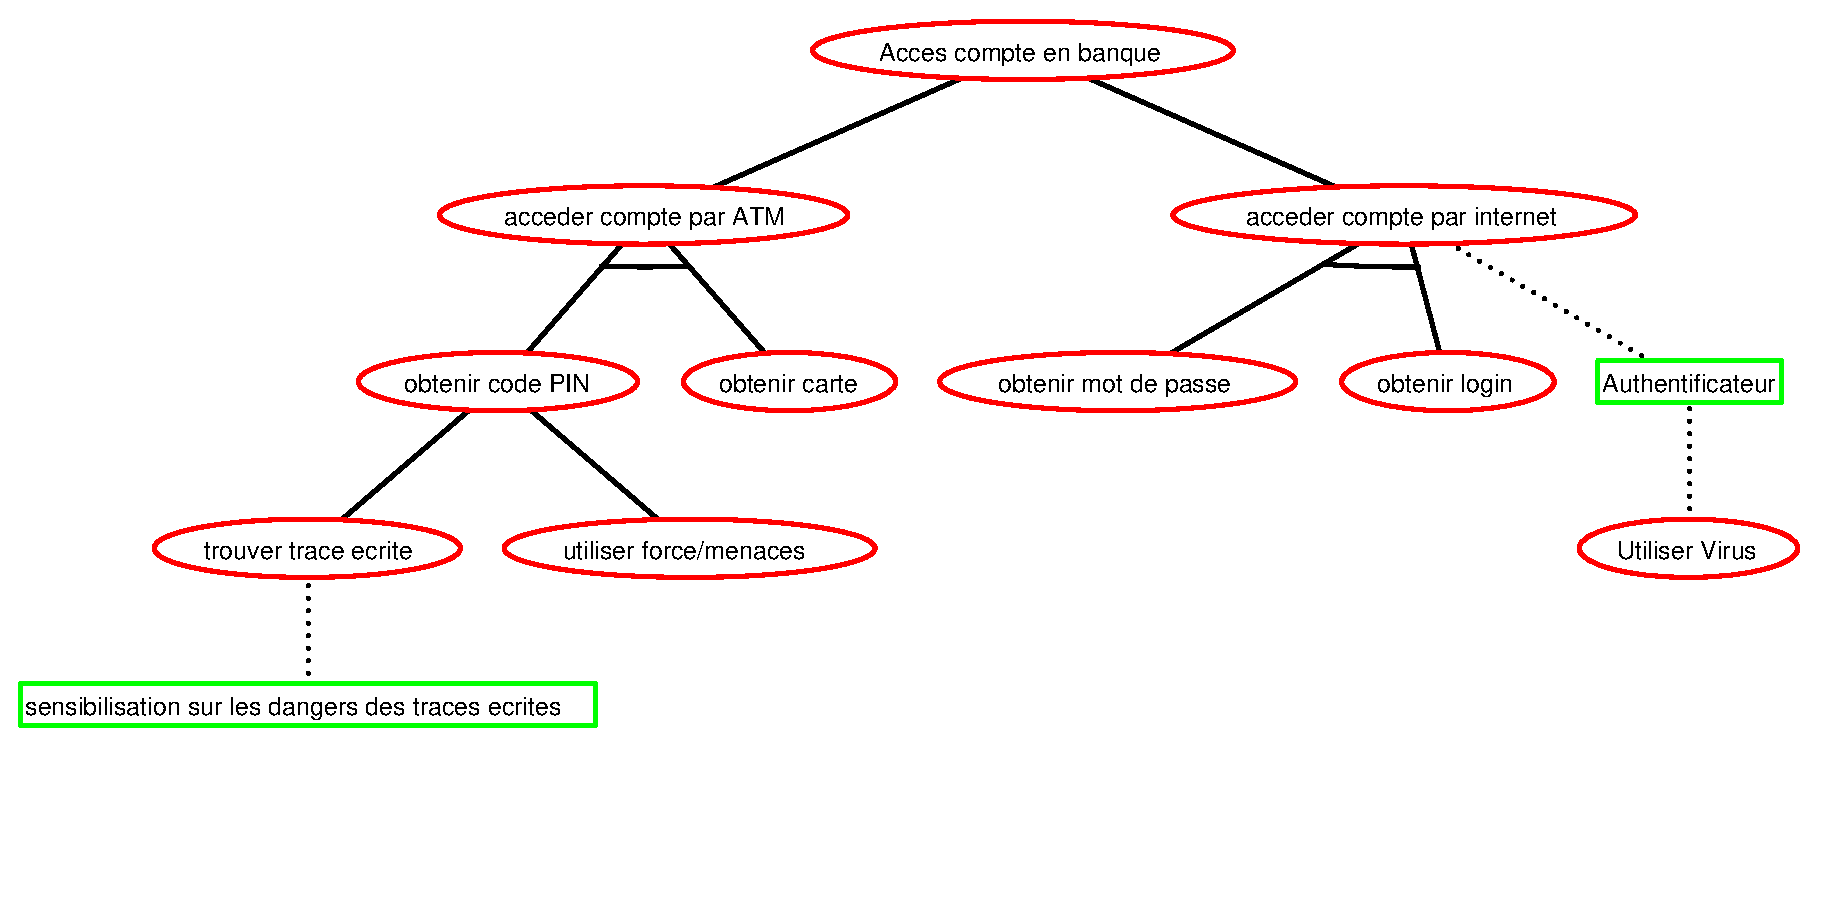
\includegraphics[width=1\textwidth]{figure/exemple2_rapport.pdf}
	        \caption{Arbre d'attaque et de défense}
	        \label{fig:arbre_exemple_3}
        \end{figure}



        \subsection{Support logiciel des ADTrees}

    
        Aujourd'hui, les arbres d'attaque sont utilisés par de nombreuses entreprises pour réaliser leurs audits de sécurité. Bien qu'il existe différents logiciels les implémentant sur le marché (SecurlTree~\cite{SecurlTree}, ATTACKTREE+~\cite{ATTACKTREE+}), de nombreuses entreprises développent en interne leur propre outil de modélisation des arbres d'attaques. Ils peuvent ainsi l'adapter au mieux à leur besoin. 

        ADTool~\cite{ADTool} est le seul logiciel que nous avons identifié à implémenter les ADTrees. Il s'agit d'un logiciel libre développé par une équipe de chercheur de l'université du Luxembourg. Mais selon nous, ce logiciel gagnerait a disposer de certaines fonctionnalités supplémentaires. Par exemple, ADTool ne prends pas en charge l'affichage simultanée de plusieurs paramètres. Il ne permets pas non plus de faire du copier-coller d'arbres. Ou encore de gérer dynamiquement la pondération des nœuds de l’arbre en fonction de l'attaquant. 

        Nous avons donc décidé de créer notre propre logiciel basé sur ADTool, l'agrémentant de fonctionnalités supplémentaires.




